\RequirePackage{luatex85}
\documentclass[tikz]{standalone}

\usetikzlibrary{decorations.pathreplacing}

\begin{document}

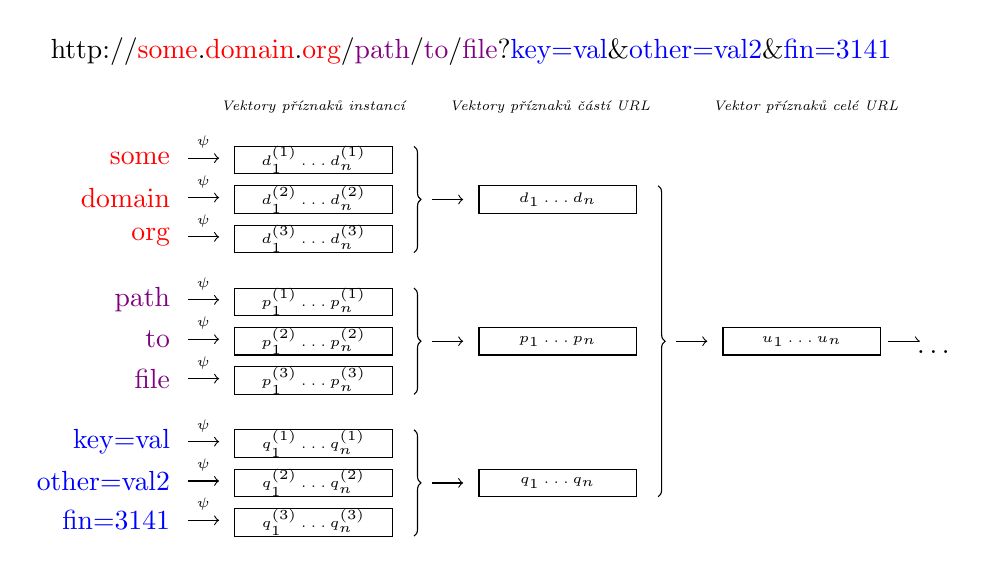
\begin{tikzpicture}
	\draw (-1, 0.5) node[anchor=north,fill=white] {http://\textcolor{red}{some}.\textcolor{red}{domain}.\textcolor{red}{org}/\textcolor{violet}{path}/\textcolor{violet}{to}/\textcolor{violet}{file}?\textcolor{blue}{key=val}\&\textcolor{blue}{other=val2}\&\textcolor{blue}{fin=3141}};
	\draw (-3.0, -0.3) node[anchor=north,fill=white] {\textit{\tiny Vektory příznaků instancí}};
	\draw (0.0, -0.3) node[anchor=north,fill=white] {\textit{\tiny Vektory příznaků částí URL}};
	\draw (3.25, -0.3) node[anchor=north,fill=white] {\textit{\tiny Vektor příznaků celé URL}};
	\draw (-4.7, -1.15) node[anchor=east, fill=white] {\textcolor{red}{some}};
	\draw (-4.7, -1.15) node[anchor=east, fill=white] {\textcolor{red}{some}};
	\draw (-4.7, -1.65) node[anchor=east, fill=white] {\textcolor{red}{domain}};
	\draw (-4.7, -2.15) node[anchor=east, fill=white] {\textcolor{red}{org}};
	\draw (-4.7, -2.95) node[anchor=east, fill=white] {\textcolor{violet}{path}};
	\draw (-4.7, -3.45) node[anchor=east, fill=white] {\textcolor{violet}{to}};
	\draw (-4.7, -3.95) node[anchor=east, fill=white] {\textcolor{violet}{file}};
	\draw (-4.7, -4.75) node[anchor=east, fill=white] {\textcolor{blue}{key=val}};
	\draw (-4.7, -5.25) node[anchor=east, fill=white] {\textcolor{blue}{other=val2}};
	\draw (-4.7, -5.75) node[anchor=east, fill=white] {\textcolor{blue}{fin=3141}};
	\draw[->] (-4.6, -1.15) -- node[above] { \tiny \( \psi \)} ++ (0.4, 0) ;
	\draw[->] (-4.6, -1.65) -- node[above] { \tiny \( \psi \)} ++ (0.4, 0);
	\draw[->] (-4.6, -2.15) -- node[above] { \tiny \( \psi \)} ++ (0.4, 0);
	\draw[->] (-4.6, -2.95) -- node[above] { \tiny \( \psi \)} ++ (0.4, 0);
	\draw[->] (-4.6, -3.45) -- node[above] { \tiny \( \psi \)} ++ (0.4, 0);
	\draw[->] (-4.6, -3.95) -- node[above] { \tiny \( \psi \)} ++ (0.4, 0);
	\draw[->] (-4.6, -4.75) -- node[above] { \tiny \( \psi \)} ++ (0.4, 0);
	\draw[->] (-4.6, -5.25) -- node[above] { \tiny \( \psi \)} ++ (0.4, 0);
	\draw[->] (-4.6, -5.75) -- node[above] { \tiny \( \psi \)} ++ (0.4, 0);
	\draw (-4, -1.0) rectangle ++(2, -0.35) node[pos=0.5] { \tiny \( d^{(1)}_1 \dots d^{(1)}_n \)};
	\draw (-4, -1.5) rectangle ++(2, -0.35) node[pos=0.5] { \tiny \( d^{(2)}_1 \dots d^{(2)}_n \)};
	\draw (-4, -2.0) rectangle ++(2, -0.35) node[pos=0.5] { \tiny \( d^{(3)}_1 \dots d^{(3)}_n \)};
	\draw (-4, -2.8) rectangle ++(2, -0.35) node[pos=0.5] { \tiny \( p^{(1)}_1 \dots p^{(1)}_n \)};
	\draw (-4, -3.3) rectangle ++(2, -0.35) node[pos=0.5] { \tiny \( p^{(2)}_1 \dots p^{(2)}_n \)};
	\draw (-4, -3.8) rectangle ++(2, -0.35) node[pos=0.5] { \tiny \( p^{(3)}_1 \dots p^{(3)}_n \)};
	\draw (-4, -4.6) rectangle ++(2, -0.35) node[pos=0.5] { \tiny \( q^{(1)}_1 \dots q^{(1)}_n \)};
	\draw (-4, -5.1) rectangle ++(2, -0.35) node[pos=0.5] { \tiny \( q^{(2)}_1 \dots q^{(2)}_n \)};
	\draw (-4, -5.6) rectangle ++(2, -0.35) node[pos=0.5] { \tiny \( q^{(3)}_1 \dots q^{(3)}_n \)};
	\draw[decoration={brace,mirror,raise=5pt},decorate] (-1.9, -2.35) -- ++(0, 1.35);
	\draw[decoration={brace,mirror,raise=5pt},decorate] (-1.9, -4.15) -- ++(0, 1.35);
	\draw[decoration={brace,mirror,raise=5pt},decorate] (-1.9, -5.95) -- ++(0, 1.35);
	\draw[->] (-1.5, -1.675) -- ++ (0.4, 0);
	\draw[->] (-1.5, -3.475) -- ++ (0.4, 0);
	\draw[->] (-1.5, -5.275) -- ++ (0.4, 0);
	\draw (-0.9, -1.5) rectangle ++(2, -0.35) node[pos=0.5] { \tiny \( d_1 \dots d_n \)};
	\draw (-0.9, -3.3) rectangle ++(2, -0.35) node[pos=0.5] { \tiny \( p_1 \dots p_n \)};
	\draw (-0.9, -5.1) rectangle ++(2, -0.35) node[pos=0.5] { \tiny \( q_1 \dots q_n \)};
	\draw[decoration={brace,mirror,raise=5pt},decorate] (1.2, -5.45) -- ++(0, 3.95);
	\draw[->] (1.6, -3.475) -- ++ (0.4, 0);
	\draw (2.2, -3.3) rectangle ++(2, -0.35) node[pos=0.5] { \tiny \( u_1 \dots u_n \)};
	\draw[->] (4.3, -3.475) -- ++ (0.4, 0);
	\draw (4.9, -3.475) node[anchor=north,fill=white] {\dots};
\end{tikzpicture}

\end{document}
